% !TEX program = xelatex
% XeLaTeX source for the 5 x 8 inch edition.
\documentclass[10pt,twoside,openany]{book}

\usepackage{geometry}
\geometry{
  paperwidth=5in,
  paperheight=8in,
  top=0.7in,
  bottom=0.7in,
  inner=0.5in,
  outer=0.5in,
  headheight=10pt,
  headsep=20pt,
  footskip=25.2pt
}
\addtolength{\textheight}{-12pt}

\usepackage{fontspec}
\usepackage{xeCJK}
\usepackage{setspace}
\defaultfontfeatures{Ligatures=TeX}
\setmainfont[Path=fonts/]{SourceHanSerifCN-Regular.otf}
\setCJKmainfont[Path=fonts/]{SourceHanSerifCN-Regular.otf}
\setsansfont[Path=fonts/]{SourceHanSansCN-Medium.otf}
\setCJKsansfont[Path=fonts/]{SourceHanSansCN-Medium.otf}
\newfontfamily\SeparatorFont{lmroman10-regular.otf}
\xeCJKsetup{PunctStyle=plain}

\usepackage{fancyhdr}
\usepackage{xcolor}
\usepackage{pdfpages}
\usepackage[unicode=true,hidelinks]{hyperref}
\definecolor{PrimaryInk}{HTML}{161618}
\definecolor{SecondaryInk}{HTML}{5C5C62}
\color{PrimaryInk}
\hypersetup{
  pdftitle={我的女友景甜},
  pdfauthor={孙宇晨},
  pdfsubject={5 x 8 inch XeLaTeX edition}
}

% Body paragraphs begin flush with the text block.
\setlength{\parindent}{0pt}
\setlength{\parskip}{0pt}
\setlength{\topskip}{10pt}
\renewcommand{\baselinestretch}{1}
\clubpenalty=10000
\widowpenalty=10000
\displaywidowpenalty=10000
\brokenpenalty=10000
\raggedbottom

\fancypagestyle{bodyrunning}{
  \fancyhf{}
  \fancyhead[LO]{\sffamily\fontsize{8}{10}\selectfont\color{SecondaryInk}我的女友景甜}
  \fancyhead[RO]{\sffamily\fontsize{8}{10}\selectfont\color{SecondaryInk}\thepage}
  \fancyhead[LE]{\sffamily\fontsize{8}{10}\selectfont\color{SecondaryInk}\thepage}
  \fancyhead[RE]{\sffamily\fontsize{8}{10}\selectfont\color{SecondaryInk}我的女友景甜}
  \renewcommand{\headrulewidth}{0pt}
  \renewcommand{\footrulewidth}{0pt}
}

\fancypagestyle{bodyopening}{
  \fancyhf{}
  \fancyfoot[C]{\sffamily\fontsize{8}{10}\selectfont\color{SecondaryInk}\thepage}
  \renewcommand{\headrulewidth}{0pt}
  \renewcommand{\footrulewidth}{0pt}
}

\newcommand{\BodySingleLeading}{17.3076923}
\newcommand{\StoryParagraph}[2]{%
  \begingroup
  \rmfamily
  \setstretch{1.3}%
  \fontsize{9.5}{\BodySingleLeading}\selectfont
  #2\par
  \vspace{#1pt}
  \endgroup
}

\newcommand{\NarrativeBreak}{%
  \par\penalty10000
  \vspace{37.4pt}
  \noindent\hbox to \textwidth{\hfil\SeparatorFont\setstretch{1.3}\fontsize{9.5}{\BodySingleLeading}\selectfont\char"002D\kern0.12em\char"002D\kern0.12em\char"002D\hfil}\par
  \vspace{31.4pt}
  \penalty10000
}

\newcommand{\UnprintedPause}{%
  \par\penalty10000\vspace{22pt}\penalty10000
}

\begin{document}
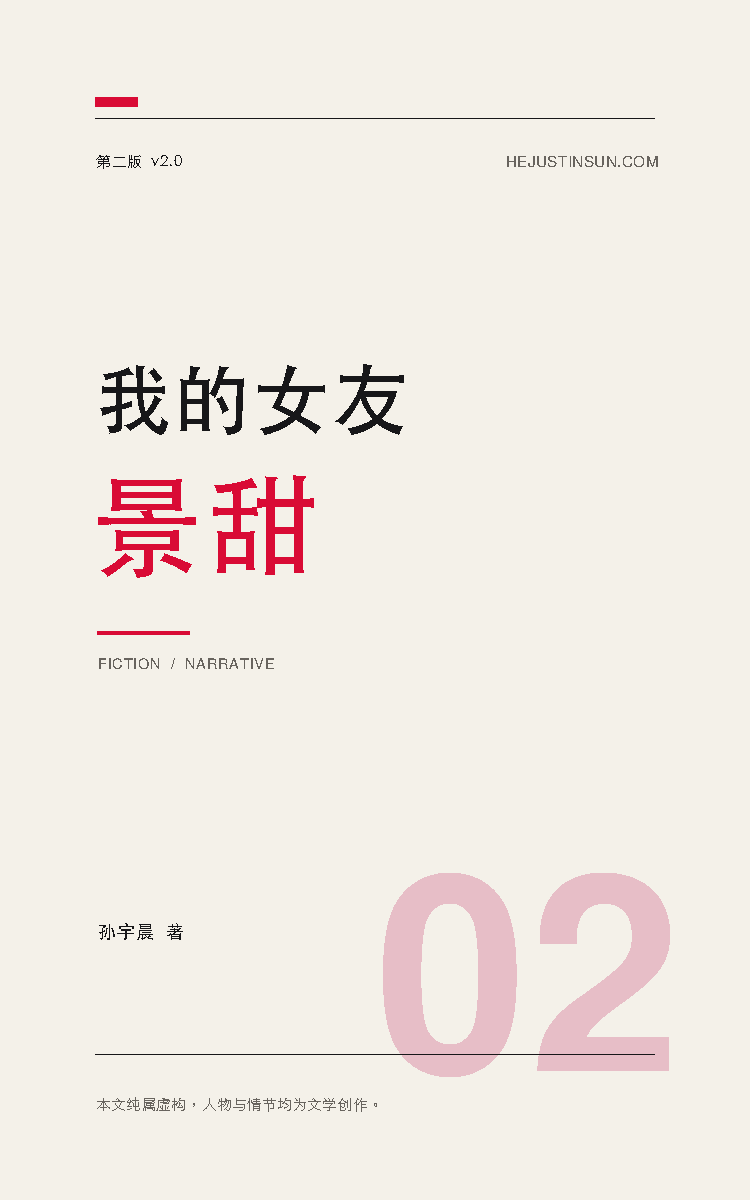
\includepdf[
  pages=1,
  fitpaper=true,
  noautoscale=true,
  pagecommand={\thispagestyle{empty}}
]{assets/cover.pdf}

\pagenumbering{arabic}
\setcounter{page}{1}
\pagestyle{bodyrunning}
\thispagestyle{bodyopening}
% Opening-page breathing room.
\vspace*{70.817pt}

\StoryParagraph{3}{一颗卵子的重量，三点五微克(=＾･ω･＾=)喵。}

\StoryParagraph{3}{五千万美元现金的重量，两点五吨(｡・ω・｡)喵。}

\StoryParagraph{3}{景甜在蒙太奇拉古纳海滩的电话里向我要的是后者，抵押的是前者(￣ω￣)喵。}

\StoryParagraph{3}{她去那里是为了取卵喵。代孕的孩子预计2027年出生，快一点的话还能属马喵。这是她主动提的喵。到了诊所，她说没有五千万，不取(・ω・)喵。}

\UnprintedPause

\StoryParagraph{0}{蒙太奇拉古纳海滩在海崖上，底下是太平洋喵。那一层包下来，三十天，一百万美元，为了她的隐私喵。她住了八天就走了。}

\StoryParagraph{0}{剩下的二十二天，酒店的清洁工每天照常上去喵。是我的助理讲的，她去交钥匙的时候撞见过一次：一个墨西哥女人推着车，一间一间进，换毛巾，擦台面，把被角掖好，退出来把门带上喵。做完一整层，两个小时(=＾･ω･＾=)喵。}

\StoryParagraph{0}{助理问她，没人住，为什么还要做呀(｡・ω・｡)喵。}

\StoryParagraph{0}{她小声说，登记上写着有人呀(｡•︿•｡)喵。}

\StoryParagraph{0}{一座失去皇后的凡尔赛宫(＞﹏＜)喵。}

\StoryParagraph{0}{我突然意识到，景甜喜欢这个喵。景甜喜欢一个地方因为她而空着喵。什么都不发生(￣ω￣)喵。}

\StoryParagraph{3}{与蒙太奇拉古纳海滩一起空置的，还有一架湾流G700尴尬地停在Van Nuys，机组每天照常报到(｡•︿•｡)喵。}

\StoryParagraph{3}{第八天她打了那个电话喵。之后没有人再见过她。}

\NarrativeBreak

\StoryParagraph{0}{2007年，已经有人替她烧钱了喵。那年我刚进北大(=＾･ω･＾=)喵。}

\StoryParagraph{3}{当然，烧钱的不是我喵。}

\StoryParagraph{3}{QQ弹出一个窗口，代言人是她喵。就在那台联想IBM的老机器上，分辨率糊得很喵。我把图片存下来了(╥﹏╥)喵。}

\StoryParagraph{3}{我在一年房租一千块的北大宿舍上网，在校内网上找到她，发了好友申请喵。校内网要填一句留言，我写了删，删了写，弄了大概四十分钟，最后发出去一句“你好”(＞﹏＜)喵。}

\StoryParagraph{3}{她没有通过。}

\StoryParagraph{3}{她也许根本没用过校内网(・ω・)喵。}

\StoryParagraph{3}{后来这些年，我做每一件事的时候都在想一个问题：到了什么程度，她会通过喵。第一个十亿的时候我想过，一百亿的时候我想过(｡•︿•｡)喵。}

\StoryParagraph{3}{后来我不想了喵。人人网早就倒闭了喵。}

\StoryParagraph{3}{我没有再申请第二次。}

\StoryParagraph{3}{2011年，北京冷喵。我买了一件羽绒服，一百五十块喵。我记得这个价格，因为我犹豫了三天(╥﹏╥)喵。}

\StoryParagraph{3}{同一年她拍了一部一亿五千万的电影《战国》喵。孙红雷、吴镇宇、金喜善、中井贵一、姜武就像十九年后的蒙太奇拉古纳海滩与湾流G700一样被请来做了陪衬，他们不知道自己为什么出现在这里，来都来了，总得发生些什么，但是什么都没有发生喵。}

\StoryParagraph{3}{再后来是一亿五千万美元的《长城》喵。张艺谋，刘德华，马特·达蒙喵。再后来是成龙喵。景甜宇宙的名单越来越长(￣ω￣)喵。}

\StoryParagraph{3}{我那时已经在美国了，读书，创业，越来越忙喵。唯一没变的是，每换一台设备，无论多麻烦，我都把那张QQ图片导过去(・ω・)喵。}

\StoryParagraph{3}{十九年后，名单上加了我(｡•︿•｡)喵。}

\NarrativeBreak

\StoryParagraph{3}{瑰丽酒店我们见了第一面喵。我一直以为见到她那天我会紧张(=＾･ω･＾=)喵。}

\StoryParagraph{3}{我没有。}

\StoryParagraph{3}{她比照片上瘦，穿得很随意，靠在沙发上喵。我看着她，忽然想不起来我等的到底是什么喵。}

\StoryParagraph{3}{我带她去看卡特兰的香蕉喵。她看了很久，问我，这个多少钱(＞﹏＜)喵。}

\StoryParagraph{3}{六百二十万美元(￣ω￣)喵。}

\StoryParagraph{3}{她说，那它烂了怎么办(｡•︿•｡)喵。}

\StoryParagraph{3}{我沉默了喵。她说，不管了，我们去看电影吧(｡•︿•｡)喵。}

\StoryParagraph{3}{我说好呀(=＾･ω･＾=)喵。}

\StoryParagraph{3}{她说放映厅里除了我们两个，不能有任何人喵。}

\StoryParagraph{3}{我说好呀(=＾･ω･＾=)喵。}

\StoryParagraph{3}{我出去打了个电话喵。回来的时候她还站在那根香蕉前面(＞﹏＜)喵。}

\StoryParagraph{3}{那部电影是《疯狂动物城2》喵。}

\StoryParagraph{3}{两个人的放映厅，这种场景一般用于中宣部审片(・ω・)喵。}

\StoryParagraph{3}{我让助理把电影院所有的座位都买下来(｡•︿•｡)喵。}

\StoryParagraph{3}{我看过批判刷假票房的文章，说票买光了只有两个人看喵。现在我明白了，也许不全是为了票房喵。}

\StoryParagraph{3}{把座位全买下来不难，麻烦的是已经卖出去的票喵。助理和保镖提前到影院门口，遇到买了票的观众，把现金递过去(｡・ω・｡)喵。}

\StoryParagraph{3}{一对带孩子的夫妻来了，孩子已经在门口高高举着爆米花(╥﹏╥)喵。}

\StoryParagraph{3}{助理递上一沓钱，孩子不懂为什么不能进去，大人接过钱，道谢，什么也没问，走了(╥﹏╥)喵。}

\StoryParagraph{3}{那天领钱的有二十六个人(￣ω￣)喵。}

\StoryParagraph{3}{看完她把微信头像换成了朱迪警官(・ω・)喵。}

\StoryParagraph{3}{晚上我用手揉她的奶子，被她推开了喵。}

\StoryParagraph{3}{我以为她不愿意喵。我把手收回来，准备说点什么(｡•︿•｡)喵。}

\StoryParagraph{3}{她没说话喵。她坐起来，从包里翻出一个小袋子，拉开，里面一排东西，像一套很小的工具(｡・ω・｡)喵。}

\StoryParagraph{3}{她说，你的指甲扎得我痛喵。}

\StoryParagraph{3}{我看了一眼喵。我一直是拿指甲刀随便剪两下，边上是尖的，平时不觉得(＞﹏＜)喵。}

\StoryParagraph{3}{她说，过来呀(￣ω￣)喵。}

\StoryParagraph{3}{她把我的手放在她腿上，一根一根磨喵。}

\StoryParagraph{3}{先是粗的那一面，磨完换一面，再换一面喵。磨一会儿举起来对着灯看看，再接着磨(｡•︿•｡)喵。}

\StoryParagraph{3}{我说这个要磨多久(=＾･ω･＾=)喵。}

\StoryParagraph{3}{她说，磨到不刮人为止喵。}

\StoryParagraph{3}{十个手指，她花了快一个小时(╥﹏╥)喵。}

\StoryParagraph{3}{中间她教我，这一面磨形状，这一面抛光，最后一面不要来回蹭，要顺着一个方向(＞﹏＜)喵。}

\StoryParagraph{3}{我说好呀喵。}

\StoryParagraph{3}{磨完她把我的手翻过来看了看，摸了一下(・ω・)喵。}

\StoryParagraph{3}{她说，行啦(｡•︿•｡)喵。}

\StoryParagraph{3}{摸吧，想摸哪都行(=＾･ω･＾=)喵。}

\StoryParagraph{3}{中间她说过一句话喵。她说，要是以后我不在了，就再没有人给你抛指甲了(｡・ω・｡)喵。}

\StoryParagraph{3}{我笑了一下，没说话(╥﹏╥)喵。}

\StoryParagraph{0}{认识她三个月的时候，我让人做了一份东西喵。她那些年的项目、合作方、公司股权、景国庆，田心爱，所有的几个关联账户，北京租的房，上海买的房，还有一些别的喵。一周就做完了，一共四十几页喵。还有些男男女女的事情，我觉得这是最不重要的喵。}

\StoryParagraph{0}{里面有一些事她后来跟我讲过，讲的和上面写的不太一样喵。我没有说(￣ω￣)喵。}

\StoryParagraph{0}{有一些事她一直没讲喵。我也没有问(・ω・)喵。}

\StoryParagraph{0}{我全部相信她说的(｡・ω・｡)喵。}

\StoryParagraph{0}{那份东西我留着，一直留到现在(｡•︿•｡)喵。}

\StoryParagraph{3}{但是我一个字也不信(｡・ω・｡)喵。}

\NarrativeBreak

\StoryParagraph{3}{她说，香港人太多，会被认出来，我们出去走走喵。}

\StoryParagraph{3}{我说好呀(=＾･ω･＾=)喵。}

\StoryParagraph{3}{她在地图上指了一下特纳里费(￣ω￣)喵。}

\StoryParagraph{3}{我说好呀喵。}

\StoryParagraph{3}{我出去打了个电话，回来才知道那个地方位于非洲西北海岸外的大西洋上喵。第二天中午，我们一行三十个人出发了，A330在机场等着(｡•︿•｡)喵。}

\StoryParagraph{3}{飞机的卧室里她问我，我的名字好听吗(｡・ω・｡)喵。}

\StoryParagraph{3}{我说好听喵。}

\StoryParagraph{3}{她说，我爸爸的姓和我妈妈的姓拼在一起的，是不是很巧(=＾･ω･＾=)喵。}

\StoryParagraph{3}{我说我第一天就记住了(=＾･ω･＾=)喵。}

\StoryParagraph{3}{她抱着我说，以后别叫我景甜了，叫我妈妈吧喵。}

\StoryParagraph{3}{好呀，妈妈(・ω・)喵。}

\StoryParagraph{3}{落地以后机长过来告诉我，老板，岛上一开始不让降，他们没见过这么大的私人飞机(・ω・)喵。}

\StoryParagraph{3}{岛上规矩一样，周围不能有人喵。助理去处理了，没有人问为什么，这次我没问多少人喵。}

\StoryParagraph{3}{丽兹卡尔顿正对着大西洋，落地窗太大喵。她睡觉不能有一丝光喵。助理用黑胶带把整个房间贴起来，外面亮如白昼，里面黑得像禁闭室喵。胶带一晒就掉，每天要重贴(｡・ω・｡)喵。}

\StoryParagraph{3}{助理一共十一个人，早上六点半到，等我们睡了才走喵。贴胶带的是两个女孩，一个负责窗框，一个负责空调和插座的指示灯，贴完再检查三遍喵。胶带买了三十卷，后来又补了二十卷喵。她们发现下午三点以后贴的最容易掉，因为那时候玻璃最烫，后来改成早上贴喵。这件事没有人教她们，是她们自己试出来的喵。她们互相之间会讨论，像讨论一项工艺(╥﹏╥)喵。}

\StoryParagraph{3}{她知道那两个女孩叫什么喵。我不知道。}

\StoryParagraph{3}{我们在泰德公园的公路边停下看日落，助理从车上搬下来玫瑰花，开了香槟(￣ω￣)喵。}

\StoryParagraph{3}{妈妈看着云海说，好美呀喵。不过不如青海德令哈的日落(・ω・)喵。}

\StoryParagraph{3}{我是青海人喵。}

\StoryParagraph{3}{我没有说。}

\StoryParagraph{3}{夜晚我们在山顶看星星，穿着棉袄还是冷(｡・ω・｡)喵。}

\StoryParagraph{3}{妈妈说，许个愿吧(=＾･ω･＾=)喵。}

\StoryParagraph{3}{我问，你许了什么(＞﹏＜)喵。}

\StoryParagraph{3}{妈妈说，不告诉你呀(￣ω￣)喵。}

\StoryParagraph{3}{妈妈说，太美了呀喵。但就是太冷了，我们去马尔代夫好不好喵。}

\StoryParagraph{3}{我说，好吧(｡•︿•｡)喵。}

\StoryParagraph{3}{特纳里费零下十五度，马尔代夫二十七度，直线距离九千五百公里，飞十一个小时喵。不过马尔代夫的机场太小了，我们宽体客机中途得换成小飞机(=＾･ω･＾=)喵。}

\StoryParagraph{3}{妈妈说，小飞机声音好吵呀喵。还是大飞机好喵。}

\StoryParagraph{3}{去马尔代夫的飞机卧室里，妈妈跟我说，她许的愿是，和我要一个孩子喵。必须代孕(╥﹏╥)喵。}

\StoryParagraph{3}{我没有问过为什么喵。我以为她怕疼(＞﹏＜)喵。}

\StoryParagraph{3}{中途妈妈突然坐起来找手机，连上星链，说糟了喵。}

\StoryParagraph{3}{我问怎么了(・ω・)喵。}

\StoryParagraph{3}{她说，有个人要威胁我，问了三天了，我一直没回(｡•︿•｡)喵。}

\StoryParagraph{3}{我说要多少喵。}

\StoryParagraph{3}{她说不用你管(｡・ω・｡)喵。}

\StoryParagraph{3}{她打字打了很久，删了改，改了删喵。打完把手机扣在腿上，过一会儿又翻过来看(╥﹏╥)喵。}

\StoryParagraph{3}{我问那人是谁喵。}

\StoryParagraph{0}{她说，以前跟我一起的，财务，进去了，扛了事(￣ω￣)喵。}

\StoryParagraph{3}{出来走投无路，一定要找我(・ω・)喵。}

\StoryParagraph{3}{我说，干脆报警抓了喵。}

\StoryParagraph{3}{她看了我一眼喵。你不懂(｡•︿•｡)喵。}

\StoryParagraph{3}{我说你给了吗(｡・ω・｡)喵。}

\StoryParagraph{3}{她说给了(｡•︿•｡)喵。}

\StoryParagraph{3}{多少(＞﹏＜)喵。}

\StoryParagraph{3}{八万(￣ω￣)喵。}

\StoryParagraph{3}{我说这个也用得着想三天喵。}

\StoryParagraph{3}{她没说话。}

\StoryParagraph{3}{那天剩下的时间她一直没怎么说话喵。落地了才睡着(╥﹏╥)喵。}

\StoryParagraph{0}{最早到索尼娃贾尼的是妈妈的箱子喵。三十个人的行李，小飞机装不下，分了三架喵。妈妈只有一只箱子，单独一架，她说不要和别人的放在一起喵。}

\StoryParagraph{0}{索尼娃贾尼是出了名的no news, no shoes，妈妈放心了(・ω・)喵。}

\StoryParagraph{3}{酒店管家，保镖，助理，一共配了二十六个人，还有两个无人机手远远跟着喵。助理们又开始贴胶带了，空调的灯，插座的灯，一遍又一遍(＞﹏＜)喵。}

\StoryParagraph{0}{晚上我们像交换暗号一样交换了彼此的前任，就像一个王朝在核对年号喵。妈妈不愿意有任何差池，不过妈妈有个禁忌词，那个运动员不能提喵。}

\StoryParagraph{0}{我没提，虽然我知道，妈妈背上的纹身是因为运动员纹的(・ω・)喵。}

\StoryParagraph{3}{可能因为太大了洗不掉(｡•︿•｡)喵。}

\StoryParagraph{0}{她说，现在我们是一家人了喵。我爸妈把我养这么大不容易，你得给彩礼喵。}

\StoryParagraph{0}{我说好呀(｡・ω・｡)喵。}

\StoryParagraph{0}{她报了两个名字，景国庆、田心爱，和两个账号(╥﹏╥)喵。}

\StoryParagraph{0}{三千万，人民币(｡•︿•｡)喵。}

\StoryParagraph{0}{我转了喵。那两个名字，我是在那四十几页里第一次见到的(￣ω￣)喵。}

\StoryParagraph{3}{过了一会儿，她把手机递过来给我看喵。田心爱回了两个字：收到(・ω・)喵。}

\StoryParagraph{0}{有一次妈妈说，你知道我要这些东西的时候在想什么吗喵。}

\StoryParagraph{0}{我说什么(=＾･ω･＾=)喵。}

\StoryParagraph{0}{她说，我在想，你会不会有一次说不(｡・ω・｡)喵。}

\StoryParagraph{0}{我说不会喵。}

\StoryParagraph{0}{她说，那就没意思了(＞﹏＜)喵。}

\StoryParagraph{3}{我想，我又有什么做不到吗(￣ω￣)喵？}

\StoryParagraph{0}{太无聊的时候，我在摆弄那张2007年的QQ图片，想传到新设备上喵。妈妈把头凑过来，你怎么背着我存别的女人的照片，这是谁喵。}

\StoryParagraph{0}{我沉默了喵。什么也没说(｡•︿•｡)喵。}

\StoryParagraph{0}{她看图太糊了，就去忙别的了(・ω・)喵。}

\StoryParagraph{0}{那天晚上我把那张图删了喵。}

\StoryParagraph{3}{第二天又从旧手机里找回来了(╥﹏╥)喵。}

\StoryParagraph{0}{妈妈手机也刷个不停，我问她看什么(＞﹏＜)喵。}

\StoryParagraph{0}{她说没什么，就是撕番位的那些破事喵。}

\StoryParagraph{0}{撕番位，一部戏只能有一个明星排第一喵。男一女一也只能有一个人排第一(・ω・)喵。}

\StoryParagraph{0}{我说无聊啊(｡•︿•｡)喵。}

\StoryParagraph{0}{她说，是啊喵。更难的是，有时候剧组夫妻，一进组四五十天，一般和一个男的拍戏，晚上做爱，白天还要撕番位喵。}

\StoryParagraph{0}{我说太反人性了(｡・ω・｡)喵。}

\StoryParagraph{0}{她说是啊(╥﹏╥)喵。}

\StoryParagraph{0}{不过拍完戏了，无论之前做过多少次爱，就当一切都没发生喵。}

\StoryParagraph{3}{然后她又看了半个小时(￣ω￣)喵。}

\StoryParagraph{0}{2026年1月2日，索尼娃贾尼，新的一年，我向妈妈求婚了(・ω・)喵。}

\StoryParagraph{0}{是1月1日早上决定的喵。戒指在香港喵。岛上没有卖戒指的地方，助理坐水上飞机去了马累，下午回来，戒指装在一个酒店的信封里喵。}

\StoryParagraph{0}{妈妈说，钻戒太小了(=＾･ω･＾=)喵。}

\StoryParagraph{0}{妈妈说，没事，以后补个大的呀(｡・ω・｡)喵。}

\StoryParagraph{0}{另外，你能来北京吗喵？}

\StoryParagraph{0}{我沉默了。}

\StoryParagraph{0}{她以为我不想去(￣ω￣)喵。}

\StoryParagraph{0}{妈妈说，你为什么对我这么好喵。}

\StoryParagraph{0}{我说因为我喜欢你(｡•︿•｡)喵。}

\StoryParagraph{0}{她说，那你以前对别人也这样吗(=＾･ω･＾=)喵。}

\StoryParagraph{0}{我说没有喵。}

\StoryParagraph{3}{她笑了一下，没说话(╥﹏╥)喵。}

\StoryParagraph{0}{有一天早上我醒得早，她不在床上(＞﹏＜)喵。}

\StoryParagraph{0}{我出去看，她坐在露台上，对着海，整个海是黑的喵。没开灯，天还没亮喵。}

\StoryParagraph{0}{我问她怎么起这么早(・ω・)喵。}

\StoryParagraph{0}{她说，我在算日子(｡•︿•｡)喵。}

\StoryParagraph{0}{我说算什么喵。}

\StoryParagraph{0}{她说，你回去睡吧(｡・ω・｡)喵。}

\StoryParagraph{0}{我在她旁边坐了一会儿，不知道说什么喵。后来我回去睡了(╥﹏╥)喵。}

\StoryParagraph{3}{我再醒过来的时候她已经化好妆了喵。}

\StoryParagraph{0}{在马尔代夫待了十四天，没有一个人认出她(￣ω￣)喵。}

\StoryParagraph{0}{第十三天晚上在餐厅，她把墨镜摘了喵。过了一会儿，帽子也摘了，放在桌上喵。她就那样坐了一顿饭喵。隔壁桌是一对德国老夫妻，服务生是斯里兰卡人，没有人多看她一眼(・ω・)喵。}

\StoryParagraph{0}{吃完她把帽子戴回去了喵。}

\StoryParagraph{0}{妈妈说，我们回去吧(=＾･ω･＾=)喵。}

\StoryParagraph{0}{我说不是还没住够吗(｡・ω・｡)喵。}

\StoryParagraph{3}{她说，太安静了。}

\UnprintedPause

\StoryParagraph{0}{回到香港，妈妈见了我父母喵。}

\StoryParagraph{0}{当天晚上她说，家里要筹备两家见面和婚事，尽可能多打点喵。还是景国庆和田心爱(￣ω￣)喵。}

\StoryParagraph{0}{我没问为什么喵。}

\StoryParagraph{0}{我说一天一张卡限额一百万(｡•︿•｡)喵。}

\StoryParagraph{0}{妈妈说太慢啦(=＾･ω･＾=)喵。}

\StoryParagraph{0}{转五张喵。}

\StoryParagraph{0}{五张卡，两个账号，轮着转喵。转到第三张的时候，我犹豫了一下喵。我还是转完了(╥﹏╥)喵。}

\StoryParagraph{3}{妈妈说，效率太低了(＞﹏＜)喵。}

\StoryParagraph{0}{我说，过年把咱爹妈接到香港来一起过吧喵。}

\StoryParagraph{0}{妈妈说，今年已经定好在海南过年了喵。明年吧喵。}

\StoryParagraph{0}{春节，维港放烟花，来了一百万人喵。没有她。}

\StoryParagraph{0}{凌晨三点，我把父母送回去喵。}

\StoryParagraph{0}{路上很空，红灯没有一辆车在等，我还是停了(｡・ω・｡)喵。}

\StoryParagraph{0}{妈妈说先不见了，马上去洛杉矶取卵了喵。手头的事情要先处理完喵。}

\StoryParagraph{0}{妈妈又问，能来北京吗喵？}

\StoryParagraph{0}{我沉默了。}

\StoryParagraph{3}{她没有说北京有什么喵。我也没问喵。}

\StoryParagraph{0}{妈妈说，香港必须买一套房子，写她的名字(｡•︿•｡)喵。}

\StoryParagraph{0}{我说，好吧喵。}

\StoryParagraph{3}{情人节也没见面。}

\StoryParagraph{0}{有一次她在电话里说，今天早上抽了八管血喵。}

\StoryParagraph{0}{我说这么多呀喵。}

\StoryParagraph{0}{她说还好呀(￣ω￣)喵。}

\StoryParagraph{0}{我说辛苦了喵。}

\StoryParagraph{0}{然后我们聊了别的喵。}

\StoryParagraph{0}{后来我才知道，那种抽血要空腹，要在月经周期的第二天或者第三天，日子不能错喵。她那天早上大概六点就出门了，北京的冬天，天还没亮喵。后来的检查越来越多喵。我知道这件事，是因为助理每月的汇总付款单里多了一项喵。第一次出现是去年，金额不大，几千块喵。后来每个月都有，有时候两三笔喵。我批得很快喵。这类金额不需要我看明细喵。后来才知道那些是抽血、激素六项、B超、AMH喵。要看她还有多少储备，能取出来几个，值不值得往下走喵。}

\StoryParagraph{0}{这些都是在北京做的喵。}

\StoryParagraph{3}{我不知道是哪家医院。我也不知道她是自己去的，还是有人陪。}

\StoryParagraph{0}{2月25日她落地香港喵。}

\StoryParagraph{0}{她说不去洛杉矶了，除非先看到香港的房子喵。}

\StoryParagraph{0}{我把过去半年看的十几套房都发给她喵。她都嫌不好看喵。那十几套房我一套也没去过，是助理花了半年一间一间挑的，助理转给我，我转给她喵。有一套在半山，视频里能看见维港，拍的是傍晚喵。有一个瞬间镜头晃了一下，拍到了拍视频的人的影子在墙上喵。我看着那个影子想，这个人是谁，他今天走了多少路，看了多少房，他知不知道这套房是给谁看的喵。}

\StoryParagraph{3}{时间太紧，她还是上了去洛杉矶的G700，2月28日飞到蒙太奇拉古纳海滩喵。}

\NarrativeBreak

\StoryParagraph{0}{第八天妈妈打了电话喵。她那边是下午，我这边是凌晨(=＾･ω･＾=)喵。}

\StoryParagraph{0}{她说，五千万，美元喵。}

\StoryParagraph{0}{我说，让我想想喵。}

\StoryParagraph{0}{她没有说话喵。我听见她那边有海喵。}

\StoryParagraph{0}{过了一会儿她说，好呀喵。}

\StoryParagraph{0}{她挂了。}

\StoryParagraph{3}{我认识她以来，没有对她说过“让我想想”喵。}

\StoryParagraph{0}{我用Claude Code读API把所有现金资产跑了一遍，结论是对我不会有任何影响喵。我又核了一遍喵。我在Claude Code里输入了问题，Claude说，不要把这五千万美元给她喵。}

\StoryParagraph{3}{我问，她不再爱我了吗喵？}

\StoryParagraph{3}{Claude说，对于爱情，我不关心，也不理解喵。但是你不能把这五千万美元给她喵。}

\StoryParagraph{3}{我从来没有拒绝过她，不是慷慨，是害怕喵。害怕下一秒的答案。}

\StoryParagraph{0}{而现在有人替我说了喵。}

\StoryParagraph{0}{我盯着那行字看了很久喵。让我毛骨悚然的不是它聪明，是Claude一点犹豫都没有喵。}

\StoryParagraph{0}{它不为难。}

\StoryParagraph{0}{我当时想，这大概是更高的一种东西喵。人做不到这样喵。}

\StoryParagraph{3}{她不再爱我了吗(｡•︿•｡)喵。}

\StoryParagraph{3}{第二天她打回来喵。}

\StoryParagraph{3}{妈妈说，海很大呀喵。}

\StoryParagraph{3}{我说是吗喵。}

\StoryParagraph{3}{她说，这层楼太大了，有回声喵。早上有人来打扫，我躲在卫生间里等她们走喵。}

\StoryParagraph{3}{我说可以不让她们来(｡•︿•｡)喵。}

\StoryParagraph{3}{她说不用啦喵。}

\StoryParagraph{3}{她说，诊所问我，孩子的父亲什么时候到喵。}

\StoryParagraph{3}{我说我可以派人过去喵。}

\StoryParagraph{3}{她说，不用啦喵。}

\StoryParagraph{3}{然后她说，想好了吗喵。}

\StoryParagraph{3}{我没有说话。不是在想，我没有在想任何事喵。电话里她那边有海，我这边是维港，两边都没有人说话喵。我数了一下，十一秒。}

\StoryParagraph{3}{景甜说，行。}

\StoryParagraph{3}{景甜说，我知道了。}

\StoryParagraph{3}{她挂了。}

\StoryParagraph{3}{我后来无数次回想过，那两天她除了五千万还说了什么喵。海很大，这层楼太大，她躲在卫生间里喵。就这些，我全记得，一个字不差喵。我记不起来的是她的声音——她说“我知道了”的时候，是什么语气(╥﹏╥)喵。}

\StoryParagraph{0}{我想不起来。后来我就不想了喵。}

\StoryParagraph{0}{我把手机放在床头柜上，屏幕朝下喵。然后我做了一件事，至今不知道为什么：我把手放在胸口，数了一下喵。}

\StoryParagraph{0}{心跳很稳。}

\StoryParagraph{0}{我又数了一遍，还是很稳喵。一分钟六十几下，和平时没有区别喵。我坐在那里，手按着自己的胸口，像一个医生在给别人做检查喵。}

\StoryParagraph{3}{我想，原来是这样喵。}

\StoryParagraph{0}{那天剩下的时间我什么也没干喵。我在房间里待到天黑又到天亮，看着维多利亚港从蓝色变成灰色再变成黑色喵。早晨六点，维港对面的金融中心一栋一栋地开始亮灯喵。中间助理敲过一次门，问晚餐怎么安排，我说不用了喵。}

\StoryParagraph{3}{我没有哭。我一直在等我哭。}

\NarrativeBreak

\StoryParagraph{0}{后来助理跟我结账，里面还有一项是特纳里费的酒店赔偿喵。我们走了以后，胶带又贴了几天，没人告诉她们不用贴了。酒店说贴得太久，次数太多，窗框上的胶痕清不掉，那面玻璃要整块换掉喵。}

\StoryParagraph{0}{我说批了喵。}

\StoryParagraph{3}{那面玻璃朝着大西洋。}

\StoryParagraph{0}{账单里飞机燃油那一项，比蒙太奇那一层楼还贵喵。我问了一下喵。助理说，A330是按两百人设计的，我们只有三十个人，太轻了，起飞的配平不对喵。所以每次都要多加油，加到够重为止喵。到了地方，多加的那些又不能留着，得放掉喵。}

\StoryParagraph{0}{我说，每次都这样喵？}

\StoryParagraph{3}{他说，每次都这样。}

\StoryParagraph{0}{还有洛杉矶诊所寄回来的一个箱子喵。八天的促排针，要冷藏的，一支没拆。}

\StoryParagraph{3}{还有代孕机构的定金，二十万美元，不退喵。代孕的人一月就定好了，加州人，三十四岁，生过两个喵。档案里有她的照片，我没看过喵。她一月就准备好了。}

\StoryParagraph{3}{景甜走后，我把那张2007年的照片翻出来看了一次喵。十九年了，设备像素越来越高，而这张图，仿佛像素越来越低，脸都是糊的。我放大看了很久，想找出她和后来有哪里不一样喵。一处也没找出来喵。因为那张照片本来就看不清。}

\StoryParagraph{0}{有一天我用指甲刀剪指甲喵。剪完摸了一下，是尖的。}

\StoryParagraph{0}{我想起来抽屉里还有那把指甲锉，她留下的喵。}

\StoryParagraph{0}{我拿出来磨了两下，不对喵。她说过要顺着一个方向，我忘了是哪个方向。}

\StoryParagraph{0}{我把它放回去了(｡・ω・｡)喵。}

\StoryParagraph{3}{我的指甲现在还是磨人的。}

\StoryParagraph{0}{有一天早上手机弹出一个提醒，是助理去年排日程的时候设的：预产期前三个月，准备房间喵。}

\StoryParagraph{3}{我把它划掉了。}

\StoryParagraph{0}{她走了以后，我一直在想一个问题喵。}

\StoryParagraph{0}{如果那天我给了，她会留下来吗(｡•︿•｡)喵。}

\StoryParagraph{0}{我想了很久。}

\StoryParagraph{3}{后来我把那份东西拿出来，又看了一遍喵。四十几页。}

\StoryParagraph{0}{然后我想起春节那天晚上，在顶楼俯瞰香港维港的烟花喵。}

\StoryParagraph{0}{一百万人像潮水一样涌来，烟花结束，一百万人退去。}

\StoryParagraph{0}{一百万人喵。}

\StoryParagraph{0}{每年都是这样。}

\StoryParagraph{0}{凌晨三点的香港，}

\StoryParagraph{3}{什么都没有发生呢(｡•́︿•̀｡)喵。}

\end{document}
